\documentclass[10pt,a4paper,UTF8]{article}
\usepackage{zclorg}
\author{emacsun}
\date{}
\title{向量空间}
\hypersetup{
 pdfauthor={emacsun},
 pdftitle={向量空间},
 pdfkeywords={},
 pdfsubject={},
 pdfcreator={Emacs 25.0.50.1 (Org mode 8.3.4)}, 
 pdflang={English}}
\begin{document}

\maketitle
\tableofcontents
\titlepic{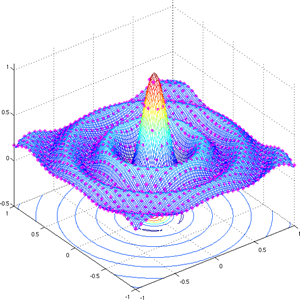
\includegraphics[scale=0.25]{../../img/sinc.PNG}}
\newpage

本文主要复习向量空间的一些基本概念和性质,包括复数的基本性质,\(\mathbf{R}^{n}\)和\(\mathbf{C}^{n}\),向量空间,子空间以及子空间的和与直和。整个内容显得有些无聊都是一些形式化的定义,但是这些定义和性质是代数的基础。

代数可以视作在集合上的运算,而在集合上定义不同的运算意味着不同的代数概念。


\section{复数的算术性质}
\label{sec:orgheadline1}


\begin{definition}
一个复数是一个有序实数对 \((a,b)\),\(a,b\in \mathbf{R}\),一般情况下我们把它记为\(a+b\mathrm{i}\),所有复数构成的集合记为\(\mathbf(C)\),即\(\mathbf{C}=\{a+b\mathrm{i},a,b\in \mathbf{R}\}\).

\(\mathbf{C}\)上的加法和乘法为:\[(a+b\mathrm{i}) + (c+d\mathrm{i}) = (a+c) + (b+d)\mathrm{i}\]\[(a+b\mathrm{i})(c+d\mathrm{i}) = (ac-bd) + (ad + bc)\mathrm{i}\]
\end{definition}

复数的算术性质:
\begin{enumerate}
\item 交换性(commutativity): 对所有的\(\alpha ,\beta \in \mathrm{C}\) 都有\(\alpha + \beta= \beta + \alpha,\alpha\beta = \beta\alpha\)
\item 结合性(associativity): 对所有的\(\alpha,\beta,\gamma \in \mathrm{C}\)都有 \((\alpha + \beta) + \gamma = \alpha + (\beta + \gamma), (\alpha\beta)\gamma = \alpha(\beta\gamma)\)
\item 单位元(identities): 对所有\(\gamma \in C\)都有 \(\gamma + 0 = \gamma,\gamma 1 =\gamma\)
\item 加法逆元(additive inverse): 对每个\(\alpha\in \mathrm{C}\)都存在唯一的\(\beta\),使得\(\alpha + \beta = 0\)
\item 乘法逆元(multiplicative inverse):对每个\(\alpha \in \mathrm{C}\)都存在唯一的\(\beta \in \mathrm{C}\)使得\(\alpha\beta = 1\)
\item 分配性质(distributive property):对所有\(\gamma,\alpha,\beta\in \mathrm{C}\)都有\(\gamma(\alpha+\beta) = \gamma\alpha + \gamma\beta\)
\end{enumerate}

\begin{definition}
定义\(\mathbf{F}^{n}\): \(\mathbf{F}^{n}\)是\(\mathbf{F}\)中元素构成的长度为\(n\)的向量的集合:\[\mathbf{F}^{n} = \{(x_{1},x_{2},\ldots,x_{n}):x_{j}\in \mathbf{F},j=1,\ldots,n\}\]对于\((x_{1},\ldots,x_{n})\in \mathbf{F}^{n}\)以及\(j\in\{1,\ldots,n\}\)称\(x_{j}\)是\(x_{1},\ldots,x_{n}\)的第\(j\)个坐标。
\end{definition}

\section{向量空间}
\label{sec:orgheadline2}


向量空间就是带有加法和标量乘法的集合\(V\),满足如下性质:
\begin{enumerate}
\item 交换性(commutativity): 对所有的\(u ,v \in \mathrm{V}\) 都有\(u + v= v + u\)
\item 结合性(associativity): 对所有的\(u,v,w \in \mathrm{V},a,b\in \mathbf{F}\)都有 \((u + v) + w = u + (v + w), (ab)v = a(bv)\)
\item 加法单位元(additive identity): 对所有\(w \in \mathbf{V}\)都有 \(0 + w =w\)
\item 加法逆元(additive inverse): 对每个\(u\in \mathrm{V}\)都存在唯一的\(v\),使得\(u + v = 0\)
\item 乘法单位元(multiplicative identity):对所有\(v\in V\)都有\(1v = v\)
\item 分配性质(distributive property):对所有\(u,v\in V; a,b\in \mathbf{F}\)都有\(a(u+v) = au + av, (a+b)v = av + bv\)
\end{enumerate}

\begin{instance}
定义\(\mathbf{F}^{\infty}\)为\(\mathbf{F}\)中元素的所有无穷序列构成的集合:\[\mathbf{F}^{\infty} = \{(x_{1},x_{2},\ldots):x_{j}\in \mathbf{F},j=1,2,\ldots\}\]
\(\mathbf{F}^{\infty}\)中标量加法和乘法的定义也和有穷序列构成的集合一样。
\end{instance}

\begin{enumerate}
\item 设\(S\)是一个集合,我们用\(\mathbf{F}^{S}\)表示从\(S\)到\(\mathbf{F}\)上所有函数的集合。
\item 对于\(f,g\in \mathbf{F}^{S}\),规定 \(f+g\in\mathbf{F}^{S}\)是如下函数:对所有\(x\in S\), \[(f+g)(x)=f(x)+g(x)\]
\item 对于\(\lambda\in \mathbf{F}\)和\(f\in \mathbf{F}^{S}\)规定\(\lambda f\in \mathbf{F}^{S}\)是如下函数:对所有的\(x\in S\),\[(\lambda f)(x)=\lambda f(x)\]
\end{enumerate}

举个例子:如果\(S\)是区间\([0,1]\),且\(\mathbf{F}=\mathbf{R}\),则\(\mathbf{R}^{[0,1]}\)是定义在区间\([0,1]\)上的所有实值函数集合。


\(\mathbf{F}^{S}\)是向量空间,且满足如下三条性质:
\begin{enumerate}
\item 若\(S\)是非空集合,则\(\mathbf{F}^{S}\)是\(\mathbf{F}\)上向量空间。
\item \(\mathbf{F}^{S}\)的加法单位元是定义如下的函数\(0:S\rightarrow \mathbf{F}:\),对所有\(x\in S\)有\[0(x) = 0\]
\item 对于\(f\in \mathbf{F}^{S}\),\(f\)的加法逆元是如下定义的函数\(-f:S\rightarrow \mathbf{F}:\) 对所有\(x\in S\),\[(-f)(x)=-f(x)\]
\end{enumerate}
\section{子空间}
\label{sec:orgheadline3}


\begin{definition}
子空间:如果\(V\)的子集\(U\)(采用与\(V\)相同的加法和标量乘法)也是向量空间,则称\(U\)是\(V\)的子空间。
\end{definition}
接下来我们给出判断向量空间的一个子集是否是子空间的最简单的方法:

\(V\)的子集\(U\)是\(V\)的子空间当且仅当\(U\)满足以下三个条件:

\begin{enumerate}
\item 加法单位元 \(0\in U\);
\item 加法封闭性 : \(u,w\in U \rightarrow u+w\in U\);
\item 标量乘法封闭性:\(a\in \mathbf{F}, u\in U \rightarrow au\in U\)
\end{enumerate}

接下来我们看看几个子空间的例子:
\begin{instance}
\begin{enumerate}
\item 若\(b\in\mathbf{F}\) 则\({(x_{1},x_{2},x_{3},x_{4})\in \mathbf{F}^{4}:x_{3}=5x_{4}+b}\)是\(\mathbf{F}^{4}\)的子空间当且仅当\(b=0\);
\item 区间\([0,1]\)上的全体实值连续函数的集合是\(\mathbf{R}^{[0,1]}\)的子空间;
\item \(\mathbf{R}\)上的全体实值可微函数的集合是\(\mathbf{R}^{\mathbf{R}}\)的子空间;
\item 区间\((0,3)\)上满足条件\(f^{'}(2)=b\)的实值可微函数的集合是\(\mathbf{R}^{(0,3)}\)的子空间当且仅当\(b=0\)
\item 极限为\(0\)的复数序列组成的集合是\(\mathbf{C}^{\infty}\)的子空间;
\end{enumerate}
\end{instance}
以上某些结论的验证表明,线性结构以微积分为基础。例如,证明第二个结论需要"两个连续函数的和仍为连续函数"。

\begin{definition}
子集的和:设\(U_{1},\ldots,U_{m}\)都是\(V\)的子集,则\(U_{1},\ldots,U_{m}\)的和定义为\(U_{1},\ldots,U_{m}\)中元素所有可能的和构成的集合,记为\(U_{1}+U_{2}+\ldots + U_{m}\),更确切的说:\[U_{1}+U_{2}+\ldots + U_{m} = \{u_{1} + \ldots + u_{m}:u_{1}\in U_{1},\ldots,u_{m}\in U_{m} \}\]
\end{definition}

\begin{instance}
接下来给一个关于子空间和的例子:假设\(U,W\)是\(\mathbf{F}^{3}\)中的子空间\(U=\{(x,0,0)\in \mathbf{F}^{3}:x\in \mathbf{F}\}\),\(W=\{(0,y,0)\in \mathbf{F}^{3}:y\in \mathbf{F}\}\),则\(U+W = \{(x,y,0):x,y\in \mathbf{F}\}\)
\end{instance}
\begin{theorem}
定理:子空间的和是包含这些子空间的最小子空间:设\(U_{1},\ldots,U_{m}\)都是\(V\)的子空间,则\(U_{1}+U_{2}+\ldots + U_{m}\)是\(V\)的包含\(U_{1},\ldots,U_{m}\)的最小子空间。
\end{theorem}
在向量空间中,子空间的和类似于集合论中子集的并,给定一个向量空间的两个子空间,包含他们的最小子空间是他们的和。类似的,给定一个集合的两个子集,包含他们的最小子集是他们的并集。
\section{子空间的直和}
\label{sec:orgheadline4}


\begin{definition}
设\(U_{1},\ldots,U_{m}\)都是\(V\)的子空间:
\begin{enumerate}
\item 和\(U_{1} + \ldots + U_{m}\)称为直和,如果\(U_{1},\ldots,U_{m}\)中的每个元素都可以唯一的表示成\(u_{1}+\ldots +u_{m}\),其中\(u_{j} \in U_{j}\)
\item 若\(U_{1} + \ldots + U_{m}\)是直和,则用\(U_{1} \oplus \ldots \oplus U_{m}\)来表示\(U_{1}+\ldots + U_{m}\)
\end{enumerate}
\end{definition}

\begin{instance}
设\(U\)是\(\mathbf{F}^{3}\)中的子空间,满足\(U=\{(x,y,0)\in \mathbf{F}^{3},x,y\in \mathbf{F}\}\), \(W\)是\(\mathbf{F}^{3}\)中的子空间,满足\(U=\{(0,0,z)\in \mathbf{F}^{3},z\in \mathbf{F}\}\),则\(\mathbf{F}^{3} = U\oplus W\)
\end{instance}
\begin{instance}
设\(U_{j}\)是\(\mathbf{F}^{n}\)中除第\(j\)个坐标以外全是\(0\)的那些向量组成的子空间,\(U_{j}=\{(0,\ldots,0,x,0,\ldots,0)\in \mathbf{F}^{n}:x\in F\}\),则\(\mathbf{F}^{n} = U_{1}\oplus \ldots \oplus U_{n}\)
\end{instance}

\begin{theorem}
设
\begin{eqnarray*}
U_{1} &=& \{(x,y,0)\in \mathbf{F}^{3}: x,y\in \mathbf{F}\} \\
U_{2} &=& \{(0,0,z)\in \mathbf{F}^{3}: z\in \mathbf{F}\} \\
U_{3} &=& \{(0,y,y)\in \mathbf{F}^{3}: y\in \mathbf{F}\} \\
\end{eqnarray*}
证明: \(U_{1} + U_{2} + U_{3}\)不是直和
\end{theorem}
\begin{proof}
显然\(\mathbf{F}^{3} = U_{1}+U_{2}+U_3\),因为每个向量\((x,y,z)\in \mathbf{F}^{3}\)都可以写成\[(x,y,z) =u_{1} + u_{2} + u_{3} =  (x,y,0) + (0,0,z) + (0,0,0)\]其中,\(u_{i}\in U_{i},i=1,2,3\)

然而\(\mathbf{F}^{3}\)不是\(U_{1},U_{2},U_{3}\)的直和,这是因为向量\((0,0,0)\)可以用两种方式写成\(u_{1} + u_{2} + u_{3}\),具体来讲我们有:
\begin{eqnarray*}
(0,0,0)&=&(0,1,0) + (0,0,1) + (0,-1,-1) \\
(0,0,0)&=&(0,0,0) + (0,0,0) + (0,0,0) 
\end{eqnarray*}
\end{proof}
直和的定义要求空间中的每个项亮都能唯一的表示成一个适当的和,然而在确定子空间的和是否是直和时,我们没有必要逐一验证。事实上,我们只需要验证\(0\)是否可以唯一的写成一个适当的和。

\begin{theorem}
设\(U_{1},\ldots,U_{n}\)都是\(V\)的子空间,则\(U_{1} + \ldots + U_{n}\)是直和,当且仅当\(0\)表示成\(u_{1} + \ldots + u_{n}\)的唯一方式是每个\(u_{j}=0,j\in\{1,\ldots,n\}\)
\end{theorem}
\begin{proof}
首先假设\(U_{1}+\ldots +U_{n}\)是直和,那么根据直和定义:如果\(0=u_{1}+\ldots + u_{n}\),则必有 \(u_{j}=0,j\in\{1,\ldots,n\}\)

现在假设:如果\(0=u_{1} + \ldots + u_{n},u_{j}\in U_{j},j\in\{1,\ldots ,n\}),则\(u_{j}=0,j\in\{1,\ldots ,n\})。为了证明\(U_{1} + \ldots + U_{n}\)是直和,设\(v\in U_{1} + \ldots + U_{n}\),我们把\(v\)写成:\[v = u_{1} + \ldots +u_{n}\]其中\(u_{j}\in U_{j},j\in \{1,\ldots ,n\}\),为了证明这个方法唯一,我们采用反证法,假设\(v\)还有一种表示\[v=v_{1} + \ldots +v_{m}\]其中\(v_{j}\in U_{j},j\in \{1,\ldots ,n\}\),把上面两种表示方式相减,则有:\[0 = (u_{1} - v_{1}) + \ldots +(u_{n} - v_{n})\]由于\(u_{i} - v_{i}\in U_{i},i\in \{1,\ldots ,n\}\),则有\(u_{i} - v_{i}=0 \rightarrow u_{i} = v_{i}, i\in\{1,\ldots ,n\}\)
\end{proof}
\begin{theorem}
设\(U\)和\(W\)都是\(V\)的子空间,则\(U+W\)是直和当且仅当\(U\cap W = \{0\}\)
\end{theorem}

\begin{proof}
证明:首先假设\(U\cap W = \{0\}\),我们来证明\(U+W\)是直和。假设\(u\in U,w\in W\)则\(0=u+w\)意味着\(u=-w\),根据向量空间的定义这说明\(u\in W\).于是\(u = U\cap W\),进而\(u=0,w=0\),所以\(0\)只能有一种表示方式,因此\(U\cap W = \{0\}\)时,\(U+W\)是直和.

然后我们证明当\(U+W\)是直和的时候,\(U\cap W = 0\). 若\(v=U\cap W\),则\(0 = v + (-v)\),其中\(v\in U,-v\in W\),由于\(0\)可以唯一的表示成\(U\)中向量和\(W\)中向量的和,我们有\(v=0\),于是\(U\cap W = 0\);

综上定理得证。
\end{proof}
\end{document}
